% 一维势能束缚态数值解(试射法)

% 未完成: 把 “数值解一维薛定谔方程(试射法)\upref{NSES} ” 合并过来

\footnote{本词条使用原子单位}我们介绍用试射法解定态薛定谔方程(TISE, Time Independent Schrodinger Equation),其中 $V(x)$ 已知
\begin{equation}
-\frac{1}{2m}\psi(x) + V(x)\psi(x) = E \psi(x)
\end{equation}
要使用 ODE 解算器(如 Matlab 的 ode45), 需要先将上式化为一阶微分方程组
\begin{equation}
\leftgroup{
\psi'(x) &= v(x)\\
v'(x) &= 2m[V(x) - E]\psi(x)
}\end{equation}

\subsection{对称势能}
先讨论偶函数势能的情况. 当 $V(x)$ 为偶函数时, 定态波函数为奇函数或偶函数. 解 ODE 应该从中点出发, 前者可用初始条件 $\psi(0)=0$, $\psi'(0)=1$, 后者可用初始条件 $\psi(0)=1$, $\psi'(0)=0$. 这样解出来的波函数一般不满足归一化条件, 需要在最后归一化.

现在可用定步长的欧拉法或者龙格库塔四阶法来解 $x\in [0, x_{max}]$ 的薛定谔方程. 显然程序中不能选取 $x\in [0,+\infty]$,但是要保证 $x_{max}$ 足够大,使解出薛定谔方程后有 $\psi(x_{max})\approx 0$, $\psi'(x_{max})\approx 0$.

\subsection{初始条件}
如果势能不是对称的, 我们一般从其中一端作为起始点解微分方程. 若某个小区间 $V(x)$ 看做常数, 解为
\begin{equation}
\psi(x) = \leftgroup{
&\sin(kx)& \quad &(E > V)\\
&\exp(\kappa x) && (E < V)
}\end{equation}
其中
\begin{equation}
k = \sqrt{2m(E - V)} \qquad
\kappa = \sqrt{2m(V - E)}
\end{equation}
所以 ODE  初始条件选择
\begin{equation}
(\psi(x_0), \psi'(x_0)) = \leftgroup{
&(0, 1)& \quad &(E > V(x_0))\\
&(\epsilon, \kappa\epsilon) && (E < V(x_0))
}\end{equation}
其中 $\epsilon$ 是一个很小的数. 第二种情况中, 解析初始条件应该是 $(0, 0)$, 但数值解中显然不能用这个. 注意最后归一化以后要检验是否两端都满足 $\psi(x_0) \ll 1$.

\subsection{甩尾法}
如何求得本征值 $E$ 呢?一种简单的方法是试射法. 顾名思义, 取不同离散的 $E$,用一定的条件判断对这些 $E$ 波函数在 $x_{max}$ 处是否满足边界条件 $\psi(x_{max}) \approx 0$\footnote{如果 $x_{max}$ 足够大,只需满足这一条件即可自动满足 $\psi'(x_{max})\approx 0$}.

一般来说,若 $E$ 略大于某本征值 $E_n$ 时,会有 $\psi(x_{max})>0$,略小时会有 $\psi(x_{max})>0$.所以画出 $\psi(x_{max})$ 关于 $E$ 的图像,用目测法找到零点即可. 若需要更精确的本征值, 可选取一个更小的区间,再次画图.

\subsection{中点匹配}
从数值误差来说,从指数末端出射时误差远远大于从指数末端入射. 所以更好的办法是从两端 $x_L, x_R$ 分别入射后在某个中点 $x_M$ 处匹配.

简单的匹配可以采用\bb{对数导数(log derivative)} 来计算匹配误差, 即
\begin{equation}
\text{err}(E) = \frac{\psi'_L(x_M)}{\psi_L(x_M)} - \frac{\psi'_R(x_M)}{\psi_R(x_M)}
\end{equation}
用多区间二分法即可得到定态能量.

但是这么做有两个缺点, 一是 $\psi(x_M)$ 为零或很小的时候, err 有可能不稳定, 二是用多区间二分法解 $\text{err}(E) = 0$ 有可能出现不收敛的解, 因为该函数存在断点(想象 $\sin(k x_M)$ 的对数导数随 $k$ 变化的情况).

为了解决这个问题, 我们可以构造一个性质更好的函数来代替对数导数, 即用 $\theta$ 表示函数 $\sin x$ 在 $x = \theta$ 处的对数导数
\begin{equation}
\theta = \Arctan(y, y')
\end{equation}
注意对数导数是关于 $\theta$ 的周期函数, 周期为 $\pi$. 只要保证两个 $\theta$ 相同或相差 $n\pi$ 就可以保证对数导数相同.

要构造关于 $\theta$ 的误差函数, 我们可以先计算两个 $\theta$ 之差
\begin{equation}
\theta = \theta_2 - \theta_1 \qquad (\theta \in [-2\pi, 2\pi])
\end{equation}
误差函数 $\opn{err}(\theta)$ 满足一些条件:
\begin{enumerate}
\item $\theta = n\pi$ 为零点(误差函数为零当且仅当对数导数相等)
\item 零点两侧异号(便于用二分法或类似算法求根)
\item 函数连续 (连续性自然是好的)
\item 周期为 $2\pi$ ($\Arctan$ 函数会使 $\theta$ 在 0 到 $2\pi$ 之间突变, 这样可以保证误差函数连续)
\end{enumerate}

一个显然的误差函数是满足这些条件的三角波(也可以用正弦函数, 但是三角波的计算量要小得多).

现在再用多区间二分法\upref{MBisec}就可以解出所有正确的束缚态能量了.

\subsection{检查漏解}
用多区间二分法时, 如果区间划分不够细, 使一个区间中存在多个解, 就会产生漏解. 检查是否漏解可以用波函数节点的数量来判断. 如果波函数的节点数是逐个递增的,则没有漏解. 也就是说第 $n$ 个能级的波函数需要有 $n - 1$ 个节点(不包括两端).

\subsection{Matlab 代码}

完整的代码(\lstinline|bnd_shoot|)见下文, 作为一个使用的例子, 我们来解一维简谐振子\upref{QSHOxn}.
\Code{bnd_shoot_demo}
结果如下
\begin{figure}[ht]
\centering
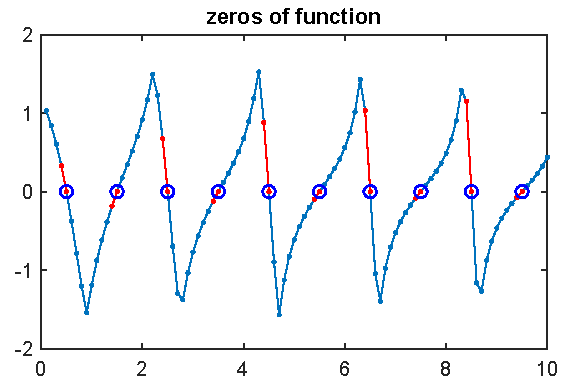
\includegraphics[width=10cm]{./figures/BndSho1.pdf}
\caption{误差函数零点} \label{BndSho_fig1}
\end{figure}

\begin{figure}[ht]
\centering
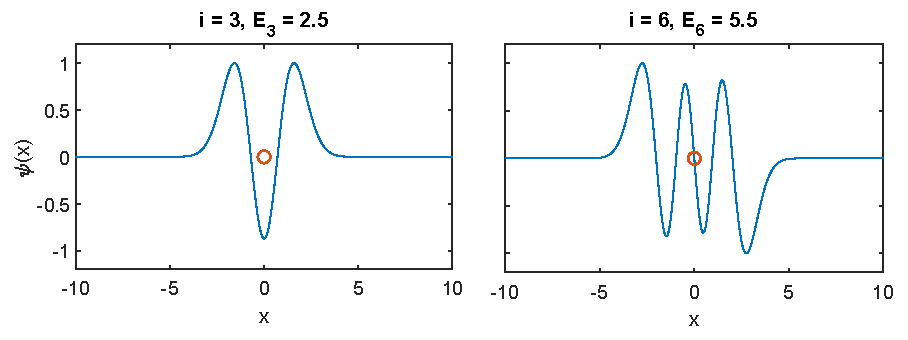
\includegraphics[width=15cm]{./figures/BndSho2.pdf}
\caption{解出的波函数, 这里只给出了第 3 和第 6 个能级, 红点表示左右波函数匹配的位置} \label{BndSho_fig2}
\end{figure}

\Code{bnd_shoot}
